 \documentclass{beamer}[10]

\usepackage{graphicx}
\usepackage{xcolor}
\usepackage{tabto}
%\usepackage{beamerthemesplit}
\usepackage{tikz}
\usepackage{cancel}
\usepackage{verbatim}
\usepackage{fancybox}
\usepackage{enumerate}
\usepackage{amsmath,amssymb,amsthm,textcomp,mathtools}
\usepackage[super]{nth}
\usepackage[amssymb]{SIunits}
\usepackage{booktabs}
\usepackage{cancel}
\usepackage{bm}
\usepackage[utf8]{inputenc}
\usepackage{tabularx}
\usepackage{ragged2e}
\newcolumntype{Y}{ >{\RaggedRight\arraybackslash}X}
\usetikzlibrary{arrows,shapes}
\newcommand\T{\rule{0pt}{2.6ex}}
\newcommand\B{\rule[-1.2ex]{0pt}{0pt}}
\definecolor{UUcrimson}{RGB}{204,0,0}
\mode<presentation>
{ \usetheme{default}
  \usecolortheme[named=UUcrimson]{structure}
  \useinnertheme{circles}
  \setbeamercovered{transparent}
  \setbeamertemplate{blocks}[rounded]
  \usefonttheme[onlymath]{serif}
  \setbeamertemplate{navigation symbols}{}
  \setbeamertemplate{footline}[page number]
  \setbeamertemplate{navigation symbols}{}
  \setbeamercolor{section in toc}{fg=black,bg=white}
  \setbeamercolor{alerted text}{fg=UUcrimson!80!gray}
  \setbeamercolor*{palette primary}{fg=white,bg=UUcrimson}
  \setbeamercolor*{palette secondary}{fg=UUcrimson!70!black,bg=gray!15!white}
  \setbeamercolor*{palette tertiary}{bg=UUcrimson!80!black,fg=gray!10!white}
  \setbeamercolor*{palette quaternary}{fg=UUcrimson,bg=gray!5!white}
  \setbeamercolor*{palette sidebar primary}{fg=UUcrimson!10!black}
  \setbeamercolor*{palette sidebar secondary}{fg=white}
  \setbeamercolor*{palette sidebar tertiary}{fg=UUcrimson!50!black}
  \setbeamercolor*{palette sidebar quaternary}{fg=gray!10!white}
  \setbeamercolor{titlelike}{parent=palette primary,fg=white}
  \setbeamercolor{frametitle}{bg=UUcrimson}
  \setbeamercolor{frametitle right}{bg=UUcrimson}
  \setbeamercolor*{separation line}{}
  \setbeamercolor*{fine separation line}{}
}

\usetikzlibrary{backgrounds}
\makeatletter
\tikzstyle{every picture}+=[remember picture]
\tikzset{%
  fancy quotes/.style={
    text width=\fq@width pt,
    align=justify,
    inner sep=1em,
    anchor=north west,
    minimum width=\linewidth,
    font=\itshape
  },
  fancy quotes width/.initial={.8\linewidth},
  fancy quotes marks/.style={
    scale=8,
    text=white,
    inner sep=0pt,
  },
  fancy quotes opening/.style={
    fancy quotes marks,
  },
  fancy quotes closing/.style={
    fancy quotes marks,
  },
  fancy quotes background/.style={
    show background rectangle,
    inner frame xsep=0pt,
    background rectangle/.style={
      fill=gray!25,
      rounded corners,
    },
  }
}
\newenvironment{fancyquotes}[1][]{%
\noindent
\tikzpicture[fancy quotes background]
\node[fancy quotes opening,anchor=north west] (fq@ul) at (0,0) {``};
\tikz@scan@one@point\pgfutil@firstofone(fq@ul.east)
\pgfmathsetmacro{\fq@width}{\linewidth - 2*\pgf@x}
\node[fancy quotes,#1] (fq@txt) at (fq@ul.north west) \bgroup}
{\egroup;
\node[overlay,fancy quotes closing,anchor=east] at (fq@txt.south east) {''};
\endtikzpicture}
\makeatother

\usepackage{scalerel}[2014/03/10]
\usepackage{stackengine}
\usepackage{empheq}
\newcommand*\widefbox[1]{\fbox{\hspace{0.5em}#1\hspace{0.5em}}}

\newcommand\reallywidetilde[1]{\ThisStyle{%
  \setbox0=\hbox{$\SavedStyle#1$}%
  \stackengine{-.1\LMpt}{$\SavedStyle#1$}{%
    \stretchto{\scaleto{\SavedStyle\mkern.2mu\sim}{.5467\wd0}}{.4\ht0}%
%    .2mu is the kern imbalance when clipping white space
%    .5467++++ is \ht/[kerned \wd] aspect ratio for \sim glyph
  }{O}{c}{F}{T}{S}%
}}
\usepackage{media9}

\logo{
\includegraphics[width=0.75cm]{logo.jpg}}
\author[Gibbs]{Dr. Jeremy A. Gibbs}
\institute{Department of Mechanical Engineering\\University of Utah}
\date{Fall 2016}
\title{LES of Turbulent Flows: Project \#1}
\begin{document}

%----------------------------------------------------------------------------------------
%	TITLE & TOC SLIDES
%----------------------------------------------------------------------------------------

\begin{frame} 
  \titlepage
\end{frame}

%------------------------------------------------

\begin{frame}
\frametitle{Overview}
\tableofcontents
\end{frame}

%------------------------------------------------
\section{Overview of Project \#1} %
%------------------------------------------------
\begin{frame}{\textit{a posteriori} studies of LES SFS models}
\begin{itemize}
	\item The ultimate test of an LES SFS model is to examine its performance in actual turbulent flow simulations
	\item Many different types of flows have been used for this purpose. Homogeneous turbulent flows are popular candidates, including
	\begin{itemize}
	\item  homogeneous shear flow
	\item rotating turbulence
	\item forced isotropic turbulence
	\item decaying isotropic turbulence
	\end{itemize}
	\item These flows are chosen for many reasons including lack of difficulties associated with filtering and modeling at boundary conditions and the relative ease (compared to more complex flows) in analyzing the resulting turbulent flow fields
\end{itemize}
\end{frame}

%------------------------------------------------
\begin{frame}{\textit{a posteriori} studies of LES SFS models}
\begin{itemize}
	\item In addition to these traditional flows used to study the performance of LES SFS models, researchers have also used simplified mathematical models
	\item On example is the stochastic Burgers equation (or Burgulence) to test models (e.g., Basu, 2009). 
	\item This offers the advantage of simple model implementation and overall low computational costs (even for DNS).
\end{itemize}
\end{frame}

%------------------------------------------------
\begin{frame}{Project Description}
\begin{itemize}
	\item The class project will be to conduct your own {\it a posteriori} study of SFS models
	\item You will do this using the provided Burgers turbulence code (Matlab). The minimum requirement will be to \underline{examine three SFS models}
	\item You will submit the assignment in the form of a short report (maximum of 4-5 pages, including references and figures)
	\item In this project, you will need to implement the models in the provided stochastic 1D Burgers equation code
\end{itemize}
\end{frame}

%------------------------------------------------
\begin{frame}{Project Description}
\begin{itemize}
	\item Don't just implement the two easiest models that you can find (the code already includes constant coefficient Smagorinsky model)
	\item Choose models based on their properties that make them ideal for your problem of interest
	\item Don't feel confined to the limited description given here and contact me if you want to do something closer to your research topic but are unsure of how to proceed
	\item The project report is due by \underline{Tuesday November 22$^{\text{nd}}$}
\end{itemize}
\end{frame}

%------------------------------------------------
\begin{frame}{Report Components}
\begin{itemize}
	\item The report should contain the following components (or equivalent)
	\item You don't need to think of this list as defining the sections of your paper, rather it offers key elements that I will be looking for
\end{itemize}
\end{frame}

%------------------------------------------------
\begin{frame}{Report Components}
\begin{itemize}
	\item A brief introduction explaining the general idea of LES and the goal of your study. You don't have to show all the LES equations, but you must include at least a description of the LES methodology. This includes a description of scale separation using a low-pass filter and the closure problem (\textit{i.e.}, what SFS stress term must be modeled). You should also briefly describe the rationale of using the 1D filtered Burgers equation as a model for the full LES equations.
\end{itemize}
\end{frame}

%------------------------------------------------
\begin{frame}{Report Components}
\begin{itemize}
	\item A description of the three models you have chosen to evaluate, including at least their general basis, any key assumptions they make, and any interesting model coefficients etc. that they use.
\end{itemize}
\end{frame}

%------------------------------------------------
\begin{frame}{Report Components}
\begin{itemize}
	\item A short description of the numerical implementation (e.g., pseudospectral methods, etc.).  The Matlab code that you will be using is based on Basu (2009) and will be discussed during the next lecture. You should make sure to mention:
\begin{itemize}
\item numerical methods used to solve the equation
\item initial conditions
\item simulation parameters that govern the evolution and initial velocity field
\item grid resolution and time step that you used for each case and the total execution time -- also specify the type of computer used and version of Matlab
\end{itemize}
\end{itemize}
\end{frame}

%------------------------------------------------
\begin{frame}{Report Components}
\begin{itemize}
	\item You should cite references when possible, although citing a reference does not completely get you off the hook from describing the code you are using.  The requirement is that an informed reader (in numerical methods and turbulence) doesn't have to check the references just to get a basic idea of your numerical treatment. I expect your description to be as brief as possible.
\end{itemize}
\end{frame}

%------------------------------------------------
\begin{frame}{Report Components}
\begin{itemize}
	\item Key results (statistical) from your study. 
\item A summary of the major findings from your study.  It is fine if these are similar results to what has been found previously or are not completely conclusive.  Still, your summary should demonstrate knowledge of the models you tested and their strengths, limitations, and any differences.
\item Any references you used in your report
\end{itemize}
\end{frame}

%------------------------------------------------
\begin{frame}{Comparison Statistics}
\begin{itemize}
	\item Your report should give as a minimum the following statistics.  
	\item Note, you are encouraged to calculate other relevant turbulence and SFS statistics depending on your application/interests and the models that you choose to study. 
	\item All statistics should be compared to statistics calculated from the provided DNS data or your own DNS run.
\end{itemize}
\end{frame}

%------------------------------------------------
\begin{frame}{Comparison Statistics}
    \begin{itemize}
	\item Evolution of the kinetic energy (KE) for the entire flow field and how it adjusts with time for each model and for at least two filter widths $\Delta$ (see Basu figure 6).
	\end{itemize}
     \begin{figure}
      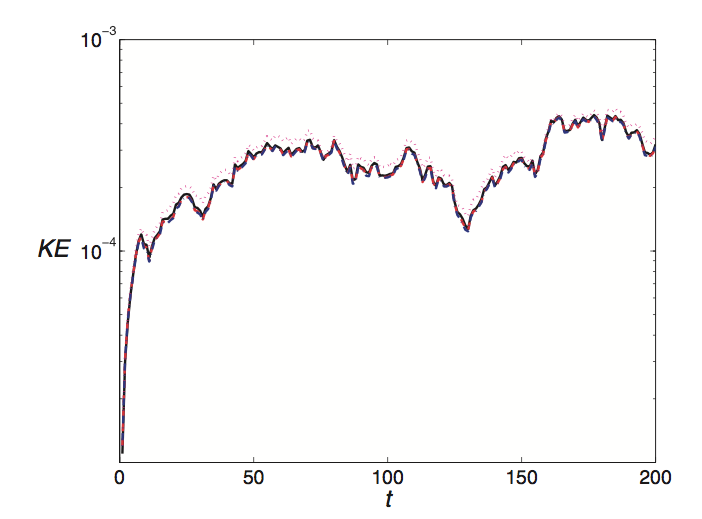
\includegraphics[width=0.7\textwidth]{basu6}
    \end{figure}
\end{frame}

%------------------------------------------------
\begin{frame}{Comparison Statistics}
    \begin{itemize}
	\item The second-order structure function and energy spectrum of the velocity both averaged over 100 time increments for each model and for at least two filter widths $\Delta$ (see Basu figure 7).
	\end{itemize}
     \begin{figure}
      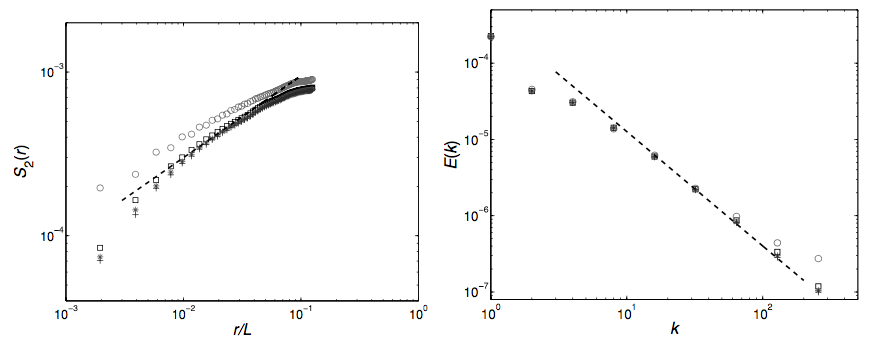
\includegraphics[width=1\textwidth]{basu7}
    \end{figure}
\end{frame}

%------------------------------------------------
\begin{frame}{Comparison Statistics}
    \begin{itemize}
	\item A plot of the temporal evolution of the mean SFS, molecular, and total energy dissipation for each of your chosen models for at least two filter widths $\Delta$ (see Basu figure 8).
	\end{itemize}
     \begin{figure}
      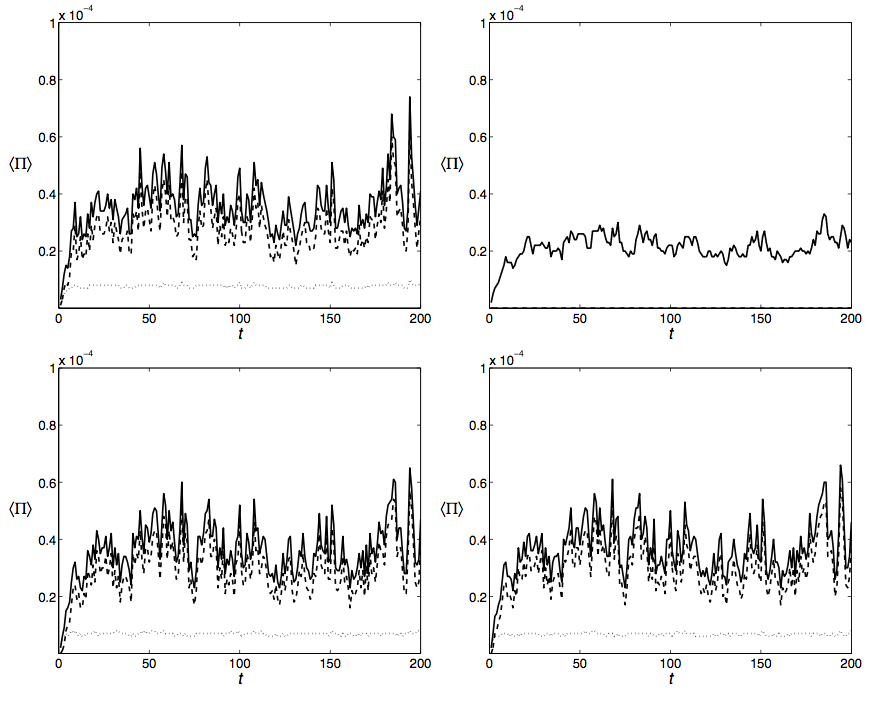
\includegraphics[width=0.75\textwidth]{basu8}
    \end{figure}
\end{frame}

%------------------------------------------------
\begin{frame}{Comparison Statistics}
    \begin{itemize}
	\item The centralized skewness and flatness factors of the velocity increments as functions of the separation distance for each tested SFS model for at least two filter widths (see Basu figures 3 and 10). 
	\end{itemize}
     \begin{figure}
      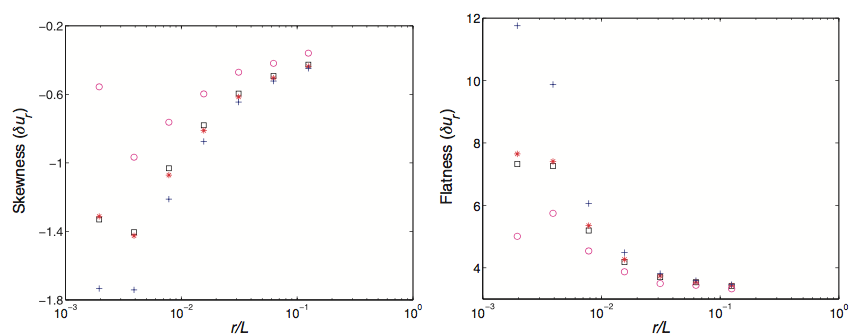
\includegraphics[width=1\textwidth]{basu10}
    \end{figure}
\end{frame}

%------------------------------------------------
\begin{frame}{Procedures}
    \begin{itemize}
	\item {\bf \underline{Procedurally}}, you will calculate your DNS statistics by first separating the velocity field into resolved and SFS components by calculating $\tilde{u}$ and $\widetilde{u^2}$ where the tilde ($\tilde{~}$) is a filter at scale $\Delta$
	\item Note, calculating $\widetilde{u^2}$ means filtering the product $u^2$
	\item Use one of the common filters discussed in class (and that you used in homework \#2) that is appropriate for the model you are comparing to.
	\item Once you have the filtered fields you can calculate the exact SFS stress tensor $\tau^{\Delta}=\widetilde{u^2}-\tilde{u}\tilde{u}$ and the exact filtered strain rate tensor (simply the filtered velocity derivative in this context)
	\end{itemize}
\end{frame}

%------------------------------------------------
\begin{frame}{Procedures}
    \begin{itemize}
	\item You will also need to calculate the other statistics listed above to compare with
	\item This is an important step when comparing LES to DNS data  to make sure that the effect of filter shape is included in the analysis (e.g., for spectra) and that you are comparing the same statistics
	\end{itemize}
\end{frame}

%------------------------------------------------
\begin{frame}{Once again, the due date}
    \begin{itemize}
	\item The project report is due by \underline{Tuesday November 22$^{\text{nd}}$}.  
	\item Please don't hesitate to contact me with any questions or problems
	\end{itemize}
\end{frame}



%------------------------------------------------



\end{document}

